\section{Simulation of Path Planner}

The same autopilot that was used for simulating the controller will be used when simulating the path planner. A path follower will be used to give course commands to the autopilot during simulation, while the rest of the states will be controlled only by the autopilot.


\subsection{Simulation Setup}

The simulation was performed using the same Simulink and Matlab setup as previously, using the path followers to generate the desired course angle. The Dubin's path that will be used as a reference is shown in figure \ref{fig:dubins_reference}.

\begin{figure}[!ht]
    \centering
    \makebox[\textwidth][c]{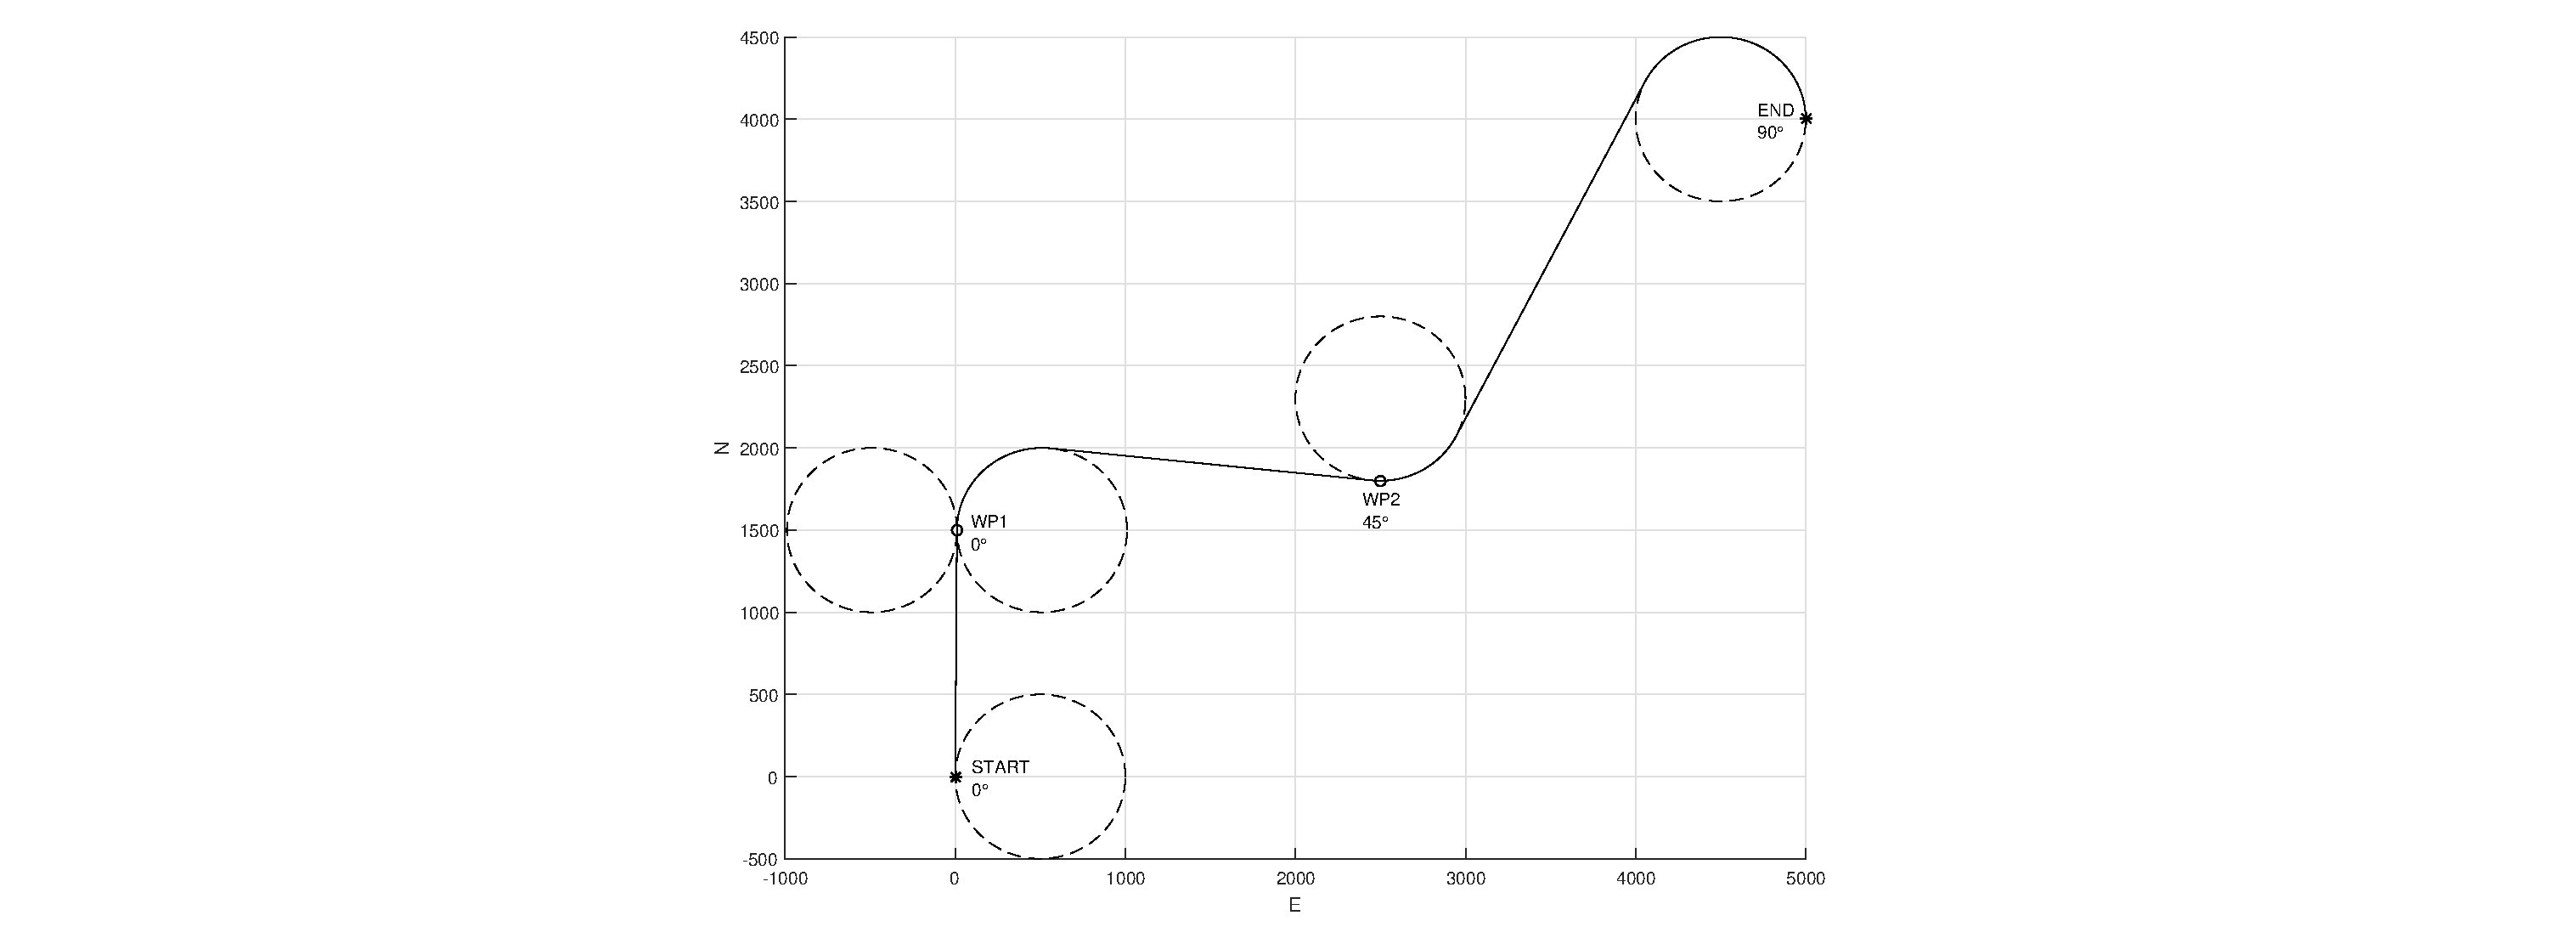
\includegraphics[width=2.2\textwidth, keepaspectratio=true]{dubins_reference.eps}}
    \caption{The path that will be simulated, with the direction associated with every waypoint.}
	\label{fig:dubins_reference}
\end{figure}

The radius of the circles in the Dubins path was chosen to $600$ m, and is the same for every waypoint. If it is assumed that there is no wind and no sideslip, the equation for a coordinated turn becomes \cite{suaBEARD}:

\begin{equation}
	R = \frac{V_g^2}{g\text{tan}(\phi)}.
\end{equation}

With $R$ set to $600$ m, and the airspeed equal to the groundspeed at $35$ m/s, the corresponding roll $\phi$ is about $15\degree$. This seems reasonable, as it is not expected that a UAV performing ground observation will be performing high dynamic maneouvres. The LOS distance was set to $200$ m by trial and failure.


\subsection{Result: Path Following}

Figure \ref{fig:first_run_path} and figure \ref{fig:first_run_turns} shows the result of the simulation when the UAV follows the generated Dubins path that is to be observed. The aircraft follows the observation path closely, and in turns it drifts slightly off and takes the outer turn. 

\begin{figure}[!ht]
    \centering
    \makebox[\textwidth][c]{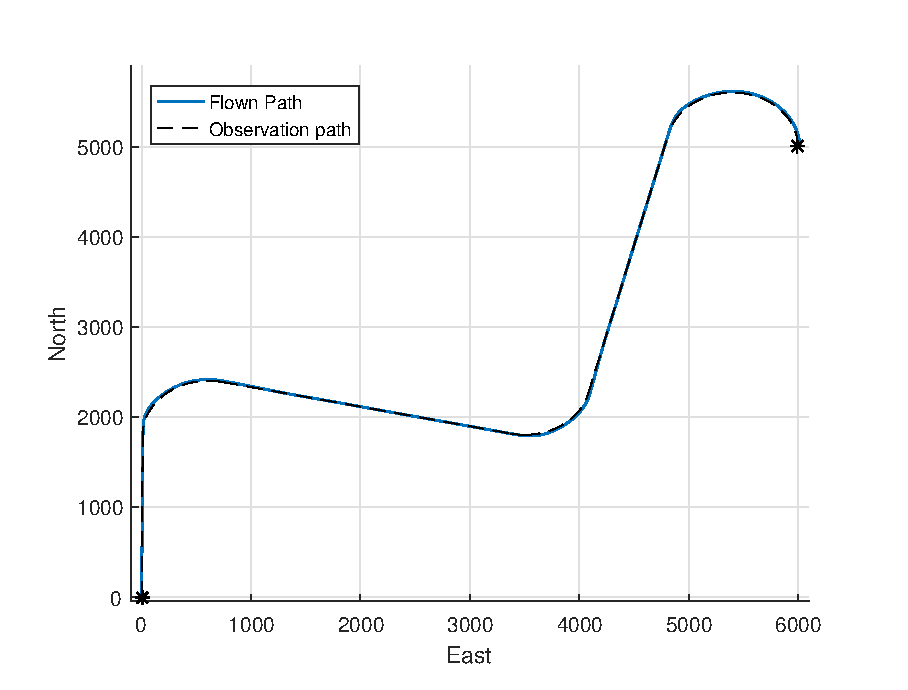
\includegraphics[width=1.2\textwidth, keepaspectratio=true]{../../results/path/first_run_path.eps}}
    \caption{The path flown by the aircraft on the first run.}
	\label{fig:first_run_path}
\end{figure}

\begin{figure}[!ht]
    \centering
    \makebox[\textwidth][c]{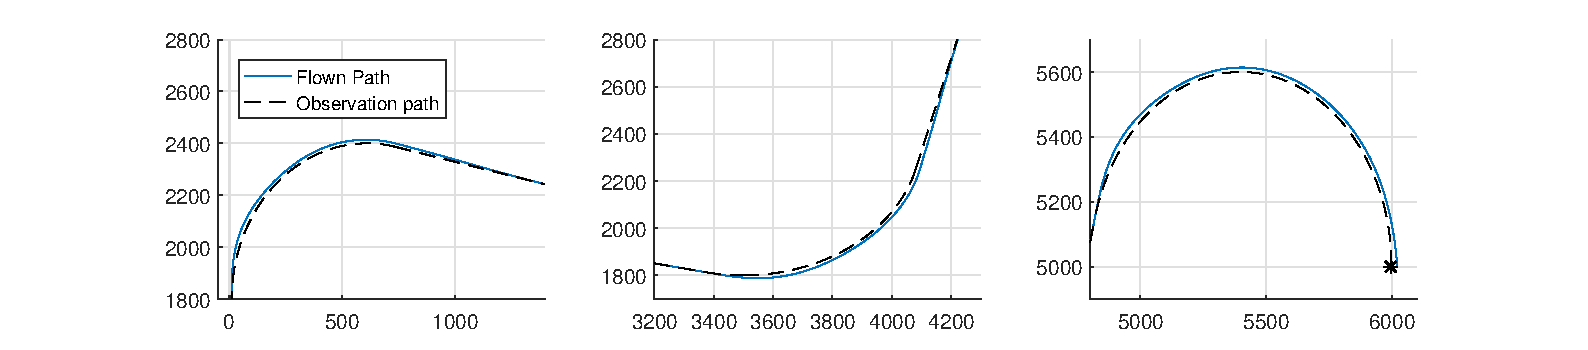
\includegraphics[width=1.8\textwidth, keepaspectratio=true]{../../results/path/first_run_turns.eps}}
    \caption{The path the aircraft took through the turns on the first run.}
	\label{fig:first_run_turns}
\end{figure}

\begin{figure}[!ht]
    \centering
    \makebox[\textwidth][c]{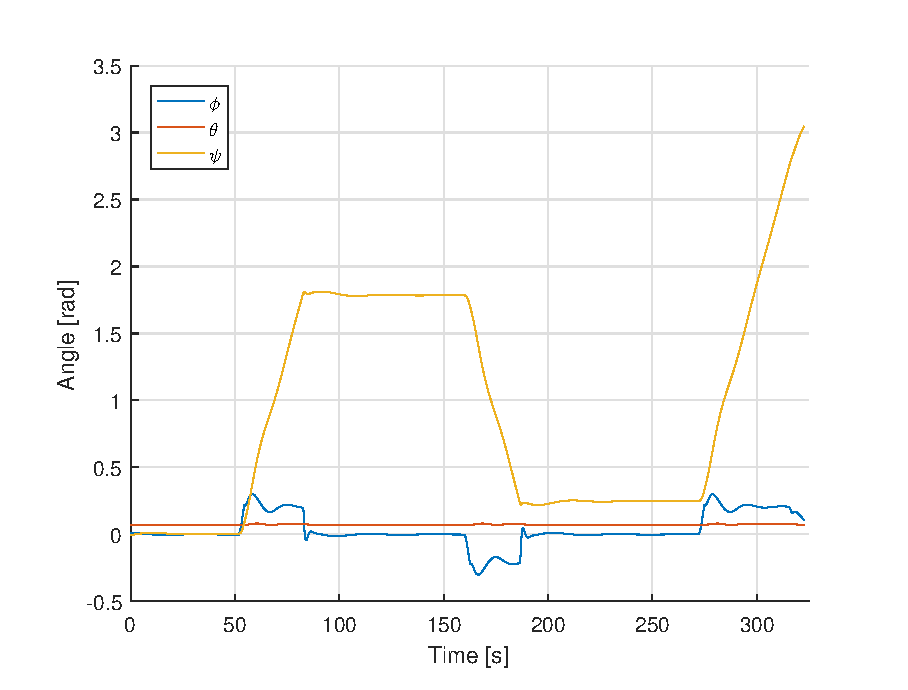
\includegraphics[width=1.2\textwidth, keepaspectratio=true]{../../results/path/first_run_states.eps}}
    \caption{The attitude states of the aircraft during the first run.}
	\label{fig:first_run_states}
\end{figure}

Figure \ref{fig:first_run_states} shows the attitude states of the aircraft during the flight, and shows that the roll $\phi$ is just below $0.25$ rad for each turn, which is about $15 \degree$ as predicted previously. However, it can be seen that $\phi$ varies during the course changes, meaning that the aircraft is not doing a perfectly smooth turn. When using equation (\ref{eq:roll_impact}) to calculate how the path should be altered, these uneven turns will cause the path to be uneven as well. The altered path is shown together with the original flown path in figure \ref{fig:altered_vs_flown}. The figure shows some "NUDGES" due to the uneven turn, mainly at the beginning and end of the turns.

\begin{figure}[!ht]
    \centering
    \makebox[\textwidth][c]{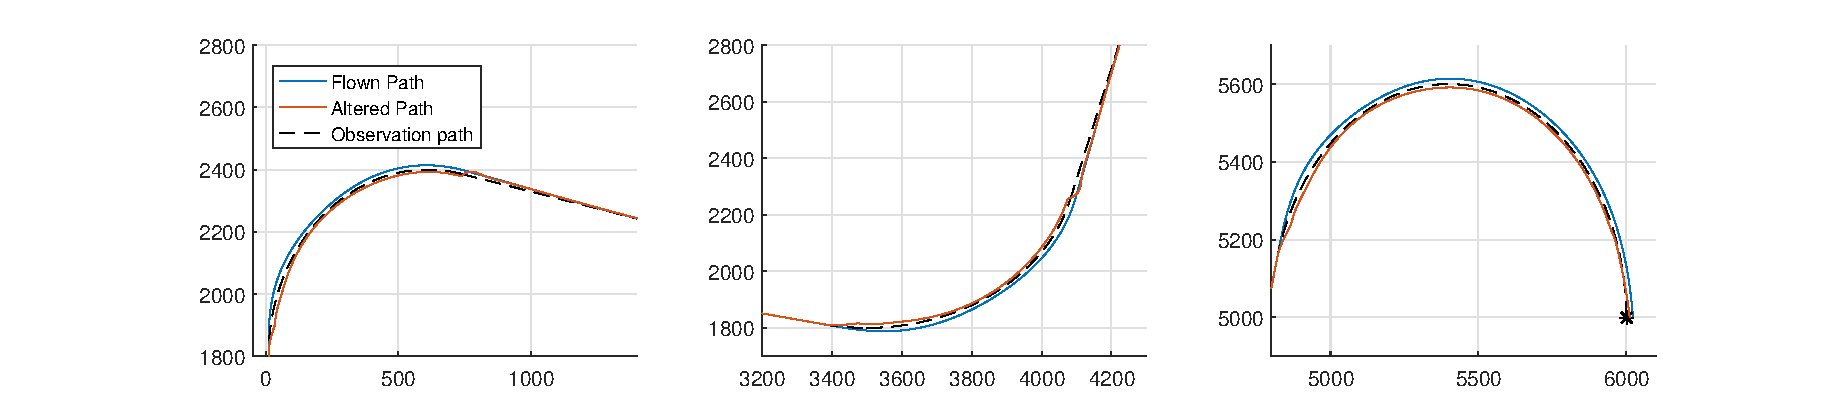
\includegraphics[width=1.8\textwidth, keepaspectratio=true]{../../results/path/altered_vs_flown.eps}}
    \caption{The figure shows how the altered path is compared to the flown path. Only the turns are shown as they are matching during the straight levelled sections.}
	\label{fig:altered_vs_flown}
\end{figure}

The altered path is supposed to counteract the slow and more constant changes in roll during a turn. The changes in roll caused by the uneven turn are much faster than than the slow changes. This means that the unwanted changes in roll can be removed by passing the signal through a low-pass filter. The result of altering the path with the low-pass filtered $\phi$ is shown in figure \ref{fig:filtered_vs_unfiltered}, and the result that the new path is smoother than the first one.

\begin{figure}[!ht]
    \centering
    \makebox[\textwidth][c]{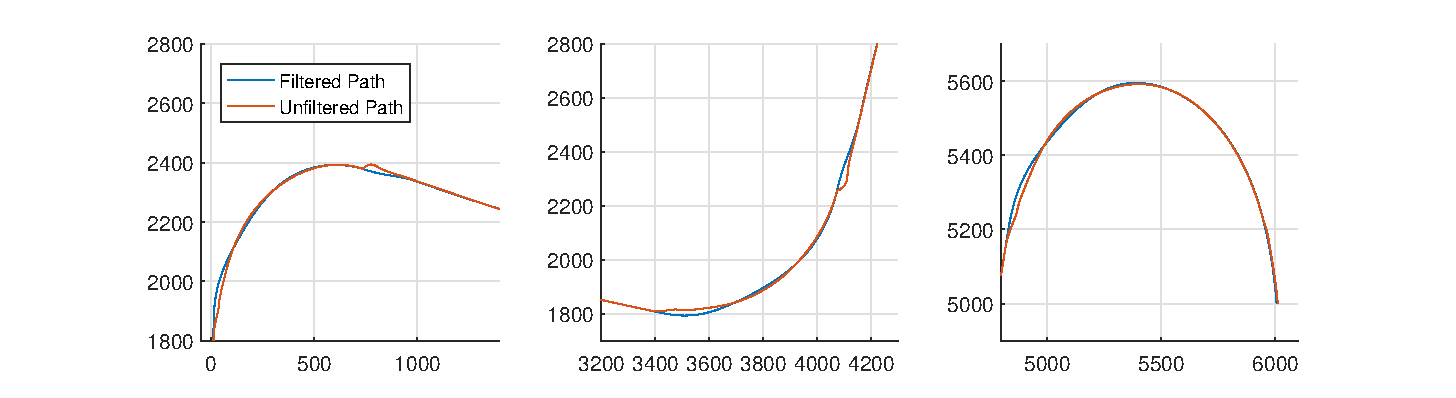
\includegraphics[width=1.8\textwidth, keepaspectratio=true]{../../results/path/filtered_vs_unfiltered.eps}}
    \caption{The path created by using the filtered signal for $\phi$ compared to using the unfiltered.}
	\label{fig:filtered_vs_unfiltered}
\end{figure}

The result of the simulation when following the altered path is shown in figures (\ref{fig:second_run_path}), (\ref{fig:second_run_turns}) and (\ref{fig:second_run_states}). It can be seen that instead of taking the outer path during turns, the aircraft now takes the inner turn which is what we want. It can be seen that $\phi$ is still uneven during turns, and about the same value as during the first run.

\begin{figure}[!ht]
    \centering
    \makebox[\textwidth][c]{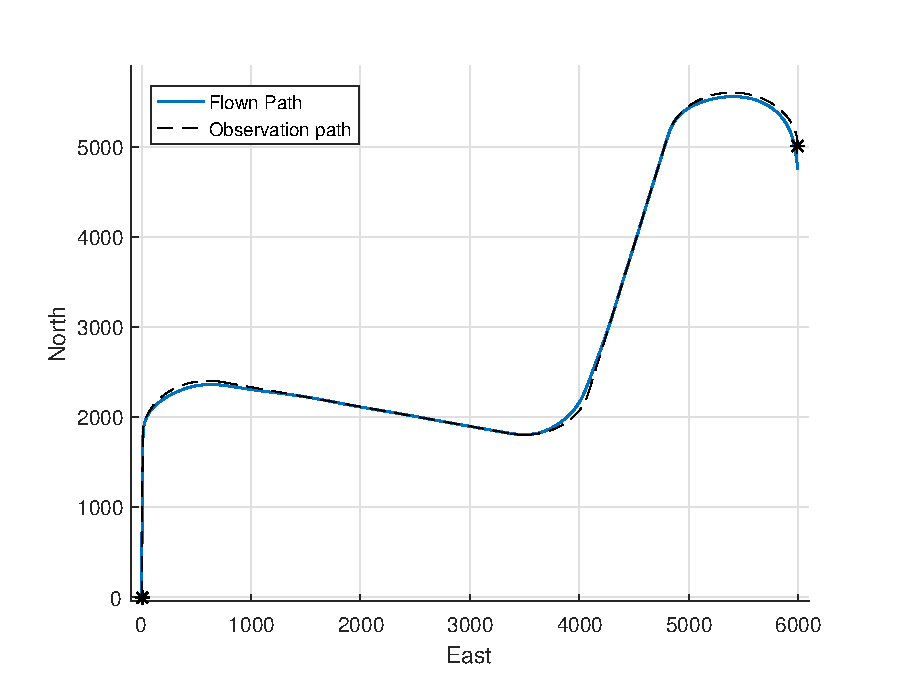
\includegraphics[width=1.2\textwidth, keepaspectratio=true]{../../results/path/second_run_path.eps}}
    \caption{The path flown by the aircraft when following the altered path.}
	\label{fig:second_run_path}
\end{figure}

\begin{figure}[!ht]
    \centering
    \makebox[\textwidth][c]{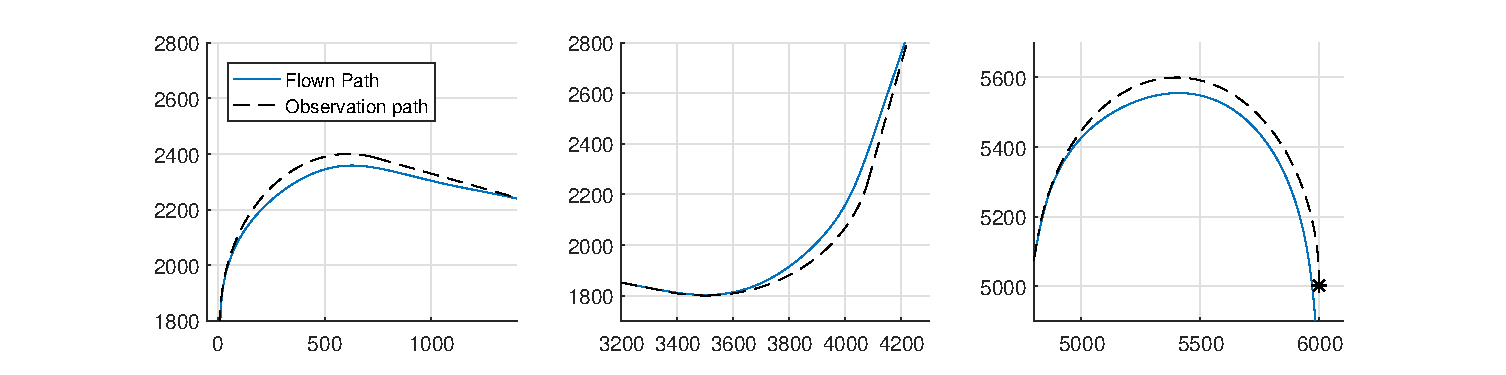
\includegraphics[width=1.8\textwidth, keepaspectratio=true]{../../results/path/second_run_turns.eps}}
    \caption{The path the aircraft took through the turns when following the altered path.}
	\label{fig:second_run_turns}
\end{figure}

\begin{figure}[!ht]
    \centering
    \makebox[\textwidth][c]{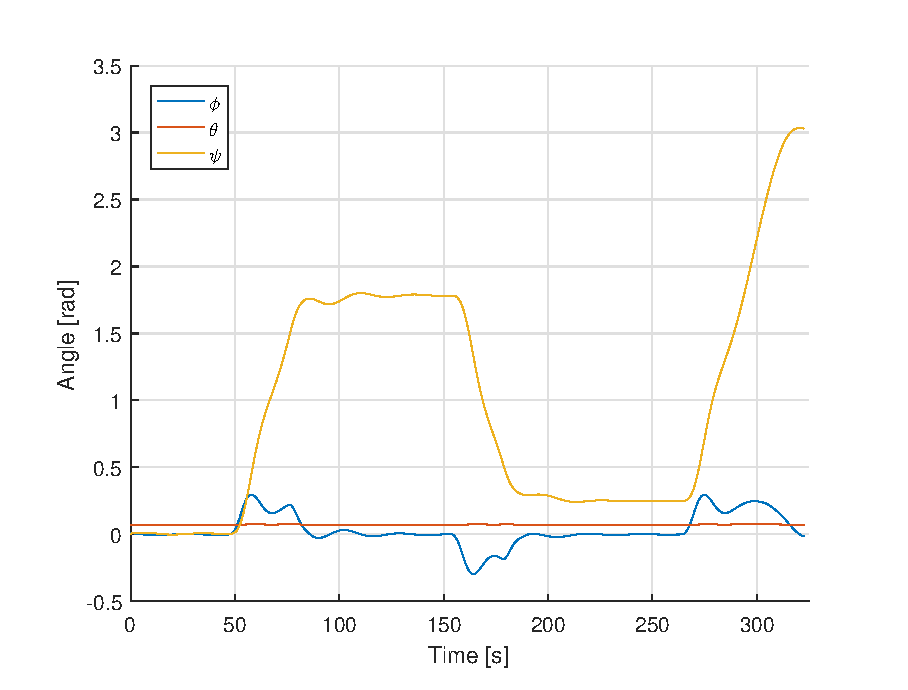
\includegraphics[width=1.2\textwidth, keepaspectratio=true]{../../results/path/second_run_states.eps}}
    \caption{The attitude states of the aircraft when following the altered path.}
	\label{fig:second_run_states}
\end{figure}


\subsection{Result: Camera Footprint}

The camera footprint for the original path is shown in figures \ref{fig:first_camera_path} and \ref{fig:first_camera_turns}. While the camera footprint is positioned fairly straight above the observation path, the observation path is outside of the camera footprint during turns. The footprint drifts completely off the observation path in the beginning of the turn, but it catches up after the initial "NUDGE". This matches the results from the previous section where the roll $\phi$ was the highest in the beginning of the turn. There is also a big change in $\phi$ at the end of the turn, which leads to a large movement of the camera footprint.

\begin{figure}[!ht]
    \centering
    \makebox[\textwidth][c]{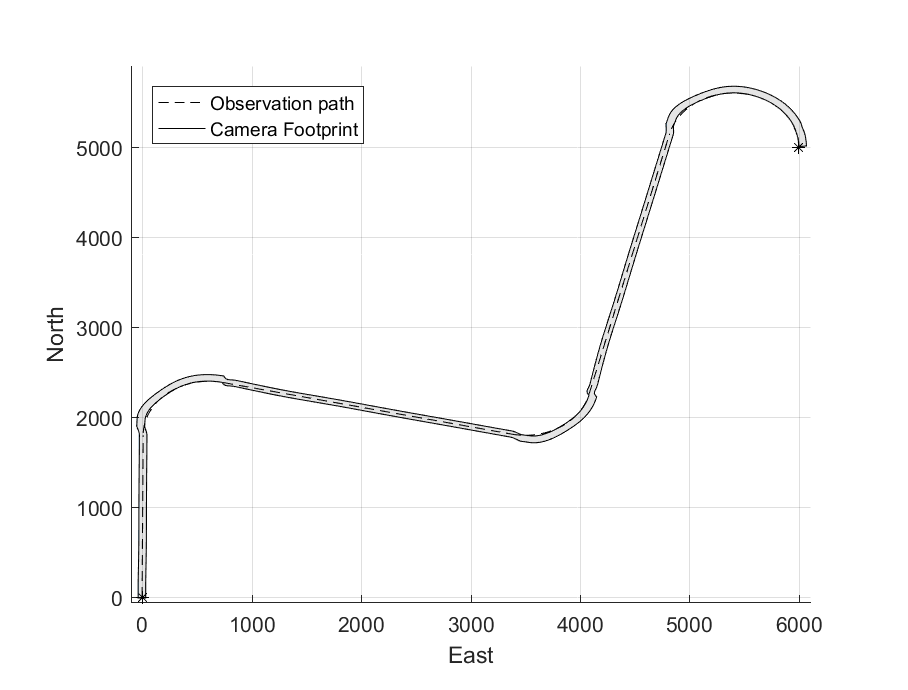
\includegraphics[width=1.2\textwidth, keepaspectratio=true]{../../results/path/first_camera_path.eps}}
    \caption{The camera footprint during simulation of the first path.}
	\label{fig:first_camera_path}
\end{figure}

\begin{figure}[!ht]
    \centering
    \makebox[\textwidth][c]{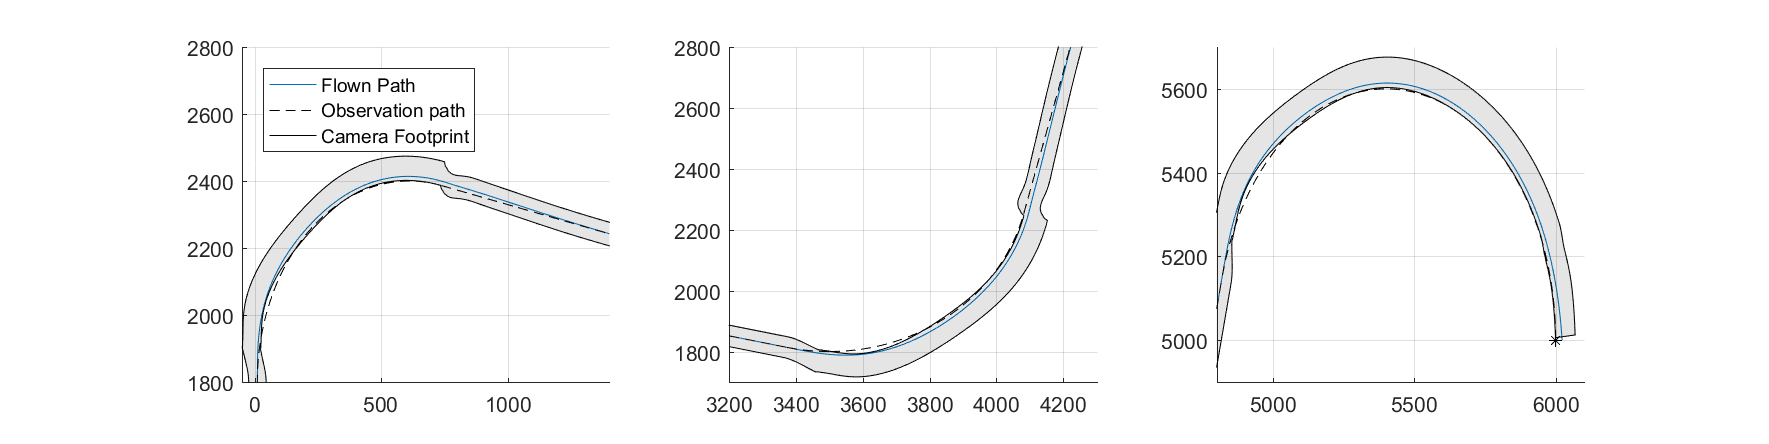
\includegraphics[width=1.8\textwidth, keepaspectratio=true]{../../results/path/first_camera_turns.eps}}
    \caption{The camera footprint in turns during the simulation of the first path.}
	\label{fig:first_camera_turns}
\end{figure}

For the altered path the camera footprint covers the observation path for the entire path as seen in figures \ref{fig:second_camera_path} and \ref{fig:second_camera_turns}. However, the observation path is not in the middle of the footprint during turns, during turns the camera footprint may drift so the observation path is only visble on the edge of the footprint.

\begin{figure}[!ht]
    \centering
    \makebox[\textwidth][c]{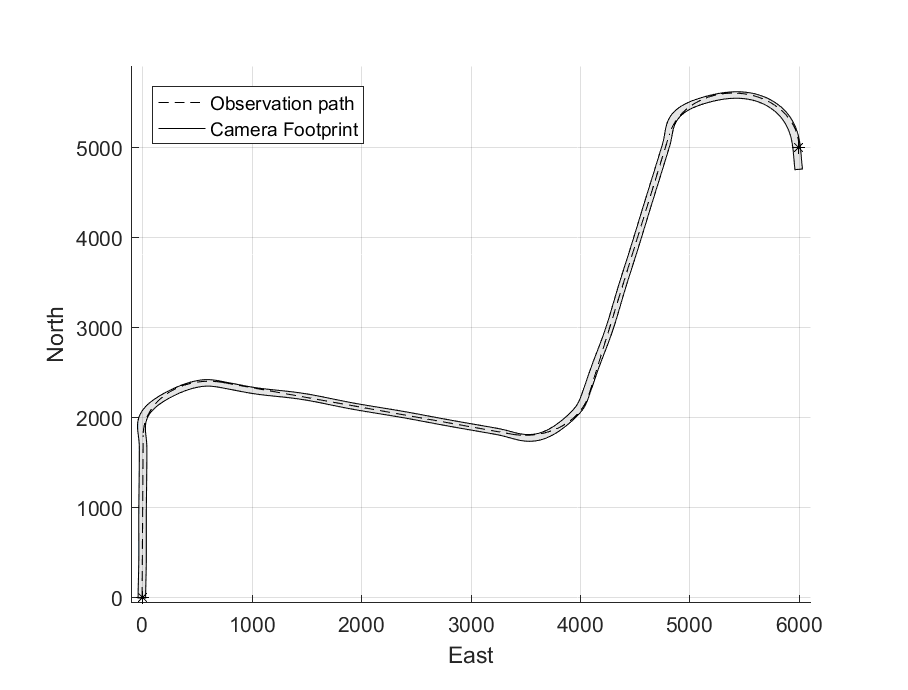
\includegraphics[width=1.2\textwidth, keepaspectratio=true]{../../results/path/second_camera_path.eps}}
    \caption{The camera footprint during simulation of the altered path.}
	\label{fig:second_camera_path}
\end{figure}

\begin{figure}[!ht]
    \centering
    \makebox[\textwidth][c]{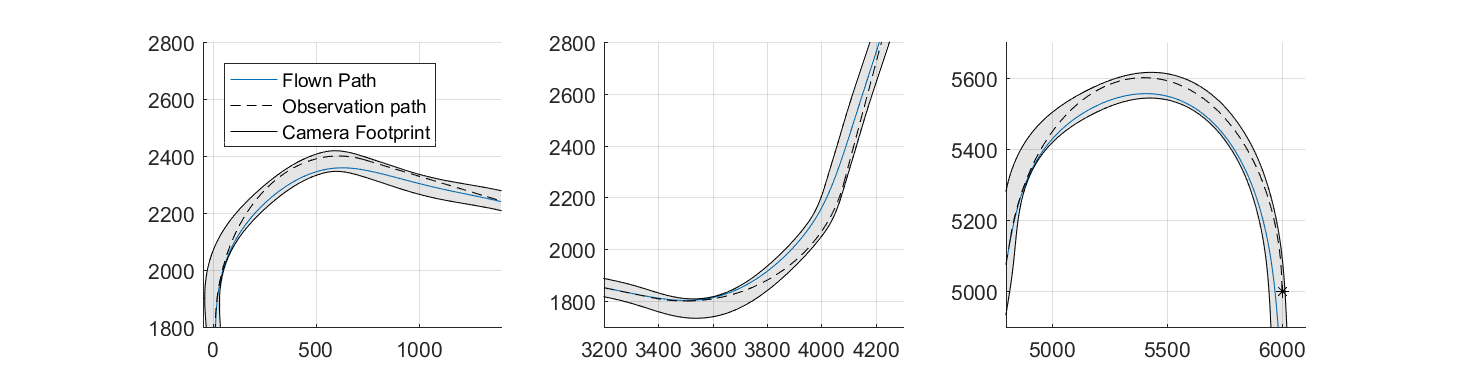
\includegraphics[width=1.8\textwidth, keepaspectratio=true]{../../results/path/second_camera_turns.eps}}
    \caption{The camera footprint in turns during the simulation of the altered path.}
	\label{fig:second_camera_turns}
\end{figure}

When the two paths are compared in figures \ref{fig:both_camera_path} and \ref{fig:both_camera_turns} the biggest difference is that the when following the original path the camera takes the outer turn, and when following the altered path it takes the inner turn. The figures also show that the altered path is smoother than the original. At the end of the two first turns for the original path the aircraft levels the wings quickly, as can be seen in figure \ref{fig:first_run_states}, which leads to a sideways shift in the camera footprint.

\begin{figure}[!ht]
    \centering
    \makebox[\textwidth][c]{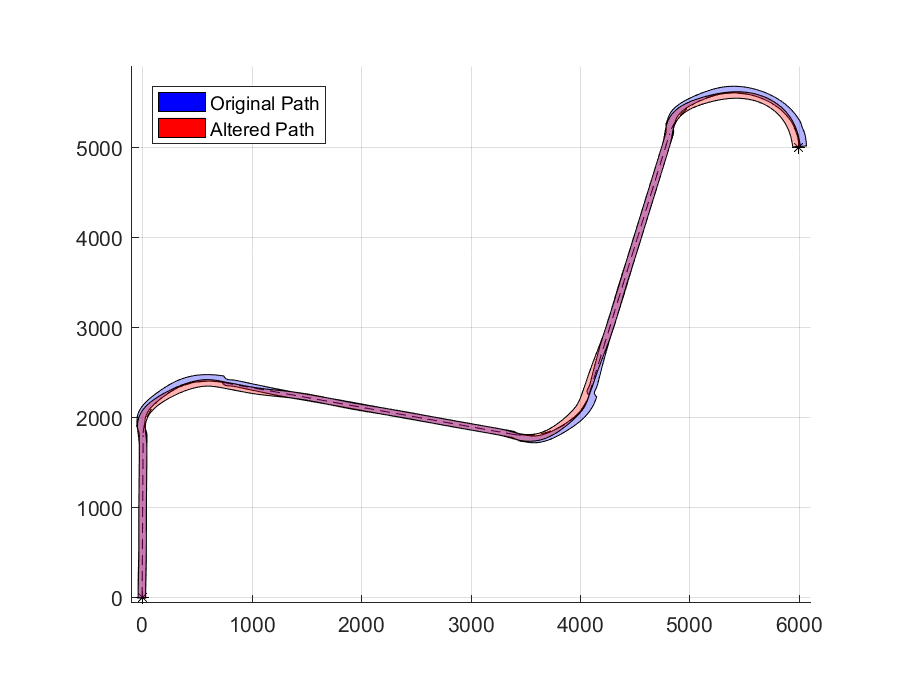
\includegraphics[width=1.2\textwidth, keepaspectratio=true]{../../results/path/both_camera_path.eps}}
    \caption{The camera footprint during simulation of the altered path.}
	\label{fig:both_camera_path}
\end{figure}

\begin{figure}[!ht]
    \centering
    \makebox[\textwidth][c]{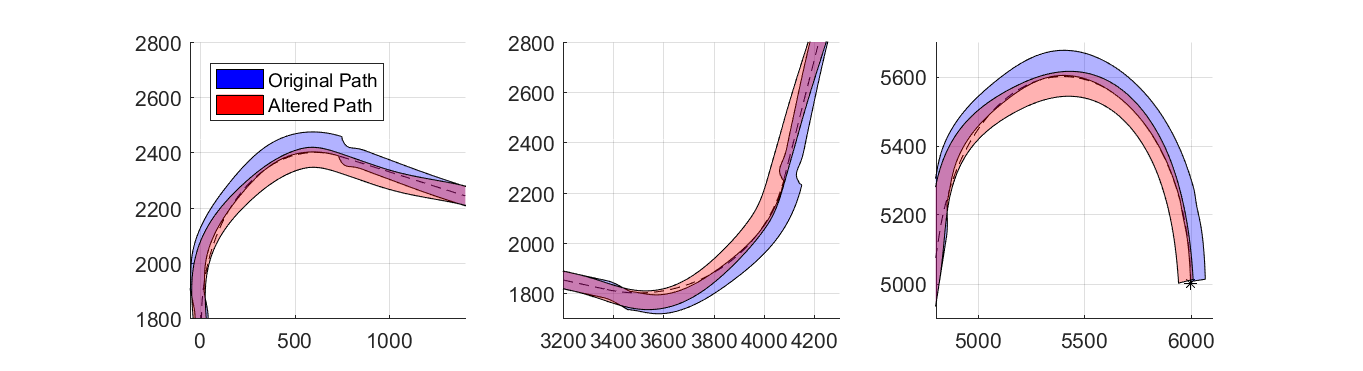
\includegraphics[width=1.8\textwidth, keepaspectratio=true]{../../results/path/both_camera_turn.eps}}
    \caption{The camera footprint in turns during the simulation of the altered path.}
	\label{fig:both_camera_turns}
\end{figure}


\subsection{Discussion}

The results of the simulation shows that the altered path does a better job observing the ground path than when trying to track the observation path. Tracking the ground path which in this case is to be observed leads to loss of information, which clearly is not acceptable in this types of mission. Another problem encountered in these simulations when tracking the observation path is rapid sideways shifts caused by a rapid change in the roll. The change between images taken during these sections is big, which most likely makes it very difficult to make good use of these images, even though the observation path has been covered.

There are also some shortcomings with the altered path used in this simulation. Even though it covered the observation path at all times, the observation path was not centered in the camera footprint. At some points during the flight, and especially in the beginning of the turns, the observation path is so close to the edge of the camera footprint that a small change in roll will most likely cause the camera to loose the ground track. One of the reasons this happens is the strategy used to alter the path. Since the path is only altered when there was roll present in the original flight path, the altered path will not start the turn any earlier than the original path did. Because the altered path cuts the corners of the original path but starts the turn at the same time, the turns of the altered path will be sharper than for the original, thus requiring a higher degree of roll. This is somewhat minimized by using a line-of-sight path follower that tracks the path ahead of the UAV, but the results show that this is not enough.


